\documentclass[10pt]{beamer}


\usetheme{metropolis}
\usecolortheme{default}
\usepackage{booktabs}
\usepackage{amsmath}
\usepackage{amssymb}
\usepackage{graphicx}
\usepackage{tikz}
\usepackage{pgfplots}
\pgfplotsset{compat=1.17}

\definecolor{myTeal}{HTML}{23373b}
\definecolor{myOrange}{HTML}{EB811B}
\setbeamercolor{alerted text}{fg=myOrange}
\setbeamercolor{frametitle}{bg=myTeal}

\title{The Economics of Bureaucracy}
\subtitle{ECO1028: Politics Without Romance}
\author{Beatriz Gietner}
\date{\today}

\begin{document}

\maketitle

\begin{frame}{Roadmap for Today}
\tableofcontents[hideallsubsections]
\end{frame}


\section{I. The Puzzle: Bureaucracy in Theory and Practice}

\begin{frame}{The Starting Point: Max Weber (1922)}

\textit{To understand the economics of bureaucracy, we first have to understand the sociological view that came before it.}

\textbf{The "Ideal Type" of Bureaucracy (4 pillars)}
\begin{itemize}
\item Hierarchy: Clear chain of command.
\item Rules: Impersonal application of law.
\item Expertise: Merit-based recruitment.
\item Neutrality: Execution of the sovereign’s will.
\end{itemize}
\alert{Bureaucracy as the most efficient administrative form. \textit{Weber, 1922, Economy and Society}}
\end{frame}


\begin{frame}{The "Ideal Type" of Bureaucracy}
\begin{center}
\includegraphics[width=0.8\linewidth]{figa.JPG}
\end{center}
Information flows up, commands flow down, and everyone follows the rules.
\end{frame}


\begin{frame}{Why Weber Saw Bureaucracy as Efficient}
\begin{itemize}
\item Specialization increases technical efficiency.
\item Rules reduce arbitrariness and corruption.
\item Professionalization improves competence.
\item Stability ensures policy continuity (even if governments change, the state continues to function).
\end{itemize}

\alert{Do you believe this to be true?}
\end{frame}

\begin{frame}{The Public Choice Departure}
\textbf{Politics Without Romance}
\begin{itemize}
\item Bureaucrats are rational individuals.
\item They respond to incentives like all economic actors.
\item Organizational behaviour emerges from individual incentives.
\end{itemize}
\end{frame}

\begin{frame}{The Central Question}
\begin{center}
\includegraphics[width=1\linewidth]{figb.JPG}
\end{center}
\end{frame}

\begin{frame}[allowframebreaks]{Why Firms and Bureaus Differ}
\begin{itemize}
\item \textbf{Firms have Residual Claimants (Owners):}
\begin{itemize}
\item \emph{Definition:} The person who keeps the surplus (profit) after costs are paid.
\item \emph{Incentive:} Strong motivation to reduce waste and maximize efficiency to increase that residual.
\end{itemize}

\item \textbf{Bureaucracies lack Residual Claimants:}
\begin{itemize}
\item No individual pockets the savings if costs are cut.
\item \emph{Result:} Weaker incentives to minimize costs ("Use it or lose it" budgets $\rightarrow$ If a bureaucrat saves 1 million by being efficient, they don't get a bonus check. In fact, usually, their budget gets cut next year because they 'obviously didn't need the money.').
\end{itemize}

\item Incentive structures therefore differ fundamentally $\rightarrow$ No profit signal, no market pricing.
\end{itemize}
\framebreak

\begin{center}
\includegraphics[width=1\linewidth]{figc.JPG}
\end{center}
\end{frame}

\begin{frame}{The Measurement Problem}
In the private sector, output is easy to measure: how many iPhones did you sell?
\begin{itemize}
\item Many public outputs are difficult to measure:
\begin{itemize}
\item National defense
\item Environmental protection
\item Judicial quality
\end{itemize}
\item Legislatures often observe budgets and activities rather than outcomes.
\begin{center}
\includegraphics[width=0.85\linewidth]{fig1.png}
\end{center}
\end{itemize}
\end{frame}



\begin{frame}[allowframebreaks]{Example: Measurement Problems in Large Public Programs}

Many government programs produce outcomes that are difficult to measure directly, making performance evaluation imperfect and creating scope for bureaucratic discretion.

\textbf{Defense spending (Mueller example):}
\begin{itemize}
\item Observable activities: troop deployment, procurement of equipment, number of missions.
\item True outcome: national security - inherently difficult to measure because it depends on events that \emph{do not occur} (deterrence).
\end{itemize}

\framebreak
\textbf{Healthcare provision (Irish HSE):}
\begin{itemize}
\item Observable activities: hospital staffing levels, procedures performed, number of beds.
\item True outcome: population health improvements and long-term patient welfare, which are influenced by many external factors (diet, exercise, and genetics) and are only partially attributable to agency performance.
\end{itemize}

\alert{When outputs are difficult to measure, monitoring relies on inputs rather than outcomes, weakening performance incentives.}

\framebreak

\begin{center}
\includegraphics[width=0.6\linewidth]{figd.JPG}
\end{center}

{Consequences of Measurement Problems:}
\begin{itemize}
\item Performance monitoring becomes costly or impossible.
\item Budget allocations become weakly tied to performance.
\item Administrative discretion (the power of government officials to make choices and apply laws flexibly) increases.
\end{itemize}
\end{frame}

\begin{frame}{The Principal–Agent Framework}
\begin{itemize}
\item Principal: Legislature or taxpayers.
\item Agent: Bureau.
\item Principal wants efficient service provision.
\item Agent has its own preferences.
\end{itemize}


\end{frame}

\begin{frame}{Information Asymmetry as the Core Friction}

Administrative agencies typically possess superior information regarding production technologies, operational constraints, and the true cost of providing services. Legislatures, in contrast, observe only proposed budgets and aggregate performance indicators.

\begin{center}
\includegraphics[width=0.85\linewidth]{fig2}
\end{center}

\textbf{Example:}
In healthcare procurement, the legislature observes the requested hospital funding level, but hospital administrators possess detailed knowledge of the true costs of staffing, equipment maintenance, and treatment delivery. This informational \textbf{asymmetry gives agencies bargaining power} during budget negotiations.

\end{frame}


\begin{frame}{Information as a Source of Power}
\begin{itemize}
\item Superior information provides bargaining leverage.
\item Hidden knowledge prevents precise legislative control.
\item Information asymmetry generates organizational autonomy.
\end{itemize}

\begin{center}
\includegraphics[width=0.8\linewidth]{fige.JPG}
\end{center}

\end{frame}

\begin{frame}{Uncertainty and Bureaucratic Authority}
\begin{itemize}
\item Authority increases when outcomes are uncertain.
\item Expertise becomes indispensable when tasks are complex.
\item Control over uncertainty translates into organizational power.
\end{itemize}


\alert{Operational Example:}
\begin{itemize}
\item Maintenance specialists understand technical systems.
\item Managers depend on their expertise.
\item Informational monopolies shift real authority away from formal hierarchy.
\end{itemize}
\end{frame}

\begin{frame}{Institutional Implication}
\begin{itemize}
\item Bureaucratic power often derives from knowledge rather than formal rules.
\item Expertise creates bargaining strength in budget negotiations.
\item Informational advantages shape agency behaviour.
\end{itemize}

\alert{From Administration to Economics:}
\begin{itemize}
\item Bureaucracies operate in environments without market discipline.
\item Incentives must therefore be analyzed institutionally.
\item Public Choice theory models bureaucratic behaviour using economic tools. 
\end{itemize}
\alert{Bureaucrats are economic actors leveraging information asymmetry in a market with no competition, not neutral implementers of rules.}
\end{frame}

\begin{frame}[allowframebreaks]{Transition: The Positive Theory of Bureaucracy}
\textbf{Concept Check: The University as a Bureau}

\begin{columns}[c]
\column{0.6\textwidth}
\textbf{The Measurement Problem:}
\begin{itemize}
\item \textbf{Output A (Research):} Easy to measure (Number of papers, citations).
\item \textbf{Output B (Teaching):} Hard to measure (Did the student actually learn? Long-term career success?).
\end{itemize}

\column{0.35\textwidth}
\begin{alertblock}{Prediction}
If the Principal (Govt) only rewards what they can measure...
\vspace{0.2cm}

\textbf{Agents (Universities) will maximize Research and ignore Teaching.}
\end{alertblock}
\end{columns}

\framebreak

 This creates the \textbf{"Multitask Problem"} (Holmstrom \& Milgrom) – a classic feature of bureaucracy: if you give a bureaucrat strong incentives (rewards or punishments) for the Easy Task, they will rationally stop doing the Hard Task completely to focus on the one that gets them rewarded.

 Holmstrom \& Milgrom’s famous conclusion is this: sometimes, it is better to have NO performance incentives than BAD ones.

If you can't measure the important stuff (Task B), you shouldn't put high-pressure incentives on the easy stuff (Task A), or you will destroy the quality of the service. This explains why many bureaucrats are paid flat salaries (low-powered incentives) rather than commissions - it prevents them from gaming the system.
\end{frame}


\section{II. The Benchmark: Niskanen (1971)}

\begin{frame}{The Objective of a Positive Theory}
\begin{itemize}
\item Bureaucracies operate outside competitive markets.
\item Standard profit-maximization models do not apply.
\item We require a behavioural model consistent with institutional realities.
\end{itemize}
\end{frame}

\begin{frame}[allowframebreaks]{Niskanen’s Core Hypothesis}
This comes from William Niskanen’s 1971 book, Bureaucracy and Representative Government. It is the 'supply and demand' model of the bureaucratic world. 
\vspace{0.3cm}
Standard economics assumes firms maximize profit. But bureaus don't have profit. So, we need a new be havioural assumption that fits the institutional reality.
\framebreak

\begin{itemize}
\item Bureaucrats maximize the size of their agency’s budget.
\item Budget size proxies for:
\begin{itemize}
\item Salary
\item Prestige
\item Career opportunities
\item Organizational influence
\end{itemize}
\end{itemize}
The bureaucrat’s utility function is tied to the size of the budget:
\[
U = f(\text{Budget})
\]
\alert{Why Is Budget Size Important?}
\begin{itemize}
\item Larger agencies justify higher managerial compensation.
\item Greater budgets expand political visibility.
\item Larger organizations increase discretionary authority.
\end{itemize}
\end{frame}

\begin{frame}{Budget Maximization Incentives}
\begin{center}
\includegraphics[width=0.9\linewidth]{figh.JPG}
\end{center}
\end{frame}

\begin{frame}{Institutional Environment}
\begin{itemize}
\item Bureau is typically a monopoly supplier.
\item Legislature acts as monopsony purchaser.
\item Absence of competitive suppliers weakens discipline.
\end{itemize}

\alert{The Bilateral Monopoly Structure:}
\begin{itemize}
\item One buyer: government.
\item One supplier: the bureau.
\item Negotiation replaces market price determination.
\end{itemize}
\alert{The Information Structure:}
\begin{itemize}
\item Bureau knows the cost function $C(Q)$.
\item Sponsor knows the benefit function $B(Q)$.
\item Cost information is not verifiable.
\end{itemize}
\end{frame}


\begin{frame}{Monopoly Supplier Position}
\begin{center}
\includegraphics[width=0.8\linewidth]{figi.JPG}
\end{center}
\end{frame}

\begin{frame}{The Sponsor’s Benefit Function}
The Sponsor represents the Legislature (and by extension, the Voter)
\[
B(Q), \quad B'(Q) > 0, \quad B"(Q) < 0
\]
\begin{itemize}
\item \textbf{Diminishing Marginal Utility:}
\begin{itemize}
\item The first unit of a public service (e.g., Police, Health) provides high value.
\item As $Q$ increases, the value of each additional unit falls ($B" < 0$).
\end{itemize}
\item \textbf{The Demand Side:}
\begin{itemize}
\item This function acts as the "Demand Curve" for the public good.
\item The Legislature is willing to pay up to the total benefit $B(Q)$.
\end{itemize}
\item \textbf{Social Efficiency Goal:}
\begin{itemize}
\item The Sponsor wants to stop where $MB = MC$ (maximum net benefit).
\end{itemize}
\end{itemize}
\end{frame}

\begin{frame}{The Bureau’s Cost Function}
The Bureau is the Monopoly Supplier
\[
C(Q), \quad C'(Q) > 0, \quad C"(Q) > 0
\]
\begin{itemize}
\item \textbf{Increasing Marginal Costs:}
\begin{itemize}
\item Costs rise more than proportionally with output ($C" > 0$).
\item Driven by scarcity of skilled labor, organizational complexity, and overtime.
\end{itemize}
\item \textbf{The Information Asymmetry:}
\begin{itemize}
\item \textbf{Critical Friction:} The true cost schedule $C(Q)$ is \emph{privately known} only by the Bureau.
\item The Sponsor cannot observe the true minimum cost of production.
\item This hidden knowledge gives the Bureau bargaining power. The Bureau can claim that costs are higher than they really are, and the politician often lacks the expertise to challenge them.
\end{itemize}
\end{itemize}
\end{frame}

\begin{frame}[allowframebreaks]{Socially Efficient Output}

The Legislature (Principal) seeks to maximize \textbf{Net Social Benefits} ($B(Q) - C(Q)$).

\[
\max_{Q} [B(Q) - C(Q)] \implies B'(Q^*) = C'(Q^*)
\]

\begin{itemize}
\item \textbf{The Optimal Point ($Q^*$):}
\begin{itemize}
\item At this level, the marginal value of the last unit equals the cost of producing it ($MB = MC$).
\item Any output beyond $Q^*$ destroys value (Deadweight Loss).
\end{itemize}
\item \textbf{The Conflict:}
\begin{itemize}
\item The Legislature wants to stop at $Q^*$.
\item The Bureau wants to push $Q$ as high as possible (until Total $B =$ Total $C$).
\end{itemize}
\end{itemize}

\framebreak
\begin{center}
\includegraphics[width=0.7\linewidth]{figf.JPG}
\end{center}
\end{frame}


\begin{frame}[allowframebreaks]{Budget Constraint in Bureau Negotiation}
\begin{itemize}
\item Bureau acts as a \textbf{Perfectly Discriminating Monopolist}.
\item It does \emph{not} sell units at a marginal price.
\item It offers a \textbf{"Take-It-Or-Leave-It"} package.
\end{itemize}

\vspace{0.5cm}

\alert{The All-or-Nothing Deal:}
\begin{itemize}
\item \textbf{The Offer:} Total Output $Q$ for Total Budget $B$.
\item \textbf{The Sponsor's Choice:} Accept the whole package or get zero service. Politician faces voters who need the service (police, health, roads), they can't say no.
\item \textbf{The Result:} The Bureau captures the entire Consumer Surplus, converting it into a larger budget.
\end{itemize}
\framebreak
\begin{center}
\includegraphics[width=0.8\linewidth]{figg.JPG}
\end{center}
\footnotesize
$Q^*$ is the efficient level.
$Q_n$ is the Niskanen level.
The Bureau pushes output way past the efficient point. The extra area on the right is Deadweight Loss - society is paying more for these extra units than they are actually worth. This is Allocative Inefficiency: The bureau is doing too much.

\end{frame}



\begin{frame}{The Budget Maximization Problem}
\[
\max B(Q) \quad \text{s.t.} \quad B(Q) \ge C(Q)
\]
\begin{itemize}
\item Bureau expands output while ensuring budget covers costs.
\end{itemize}
\alert{First-Order Condition:}
\[
(1+\lambda)B'(Q)=\lambda C'(Q)
\] $\rightarrow$ Constraint is binding (check full derivation at the end)
\begin{itemize}
\item Implies $B'(Q) < C'(Q)$ at equilibrium $\rightarrow$At the point where the bureau stops, the marginal value of the last thing they did ($B'$) is less than what it cost to produce ($C'$). They are producing "junk" units at the margin just to keep the budget large. This is the definition of economic waste.
\item Does the bureau always get away with this? That depends on Elasticity ($\eta$). In plain English: can the politician say "no"?
\end{itemize}
\end{frame}

\begin{frame}{The Role of Demand Elasticity}
If the Bureau sets a unit price $P$, the budget is $B(P)=P\cdot Q(P)$.
\[
\frac{dB}{dP}=Q+P\frac{dQ}{dP} \implies \text{Revenue change depends on } \eta
\]

\textbf{The Power of Essential Services:}
\begin{itemize}
\item \textbf{Elastic Demand ($\eta > 1$):} If the Sponsor is price-sensitive (e.g., parks, culture), raising prices ($P\uparrow$) \emph{reduces} the total budget ($B\downarrow$). The Bureau is disciplined by demand.
\item \textbf{Inelastic Demand ($\eta < 1$):} If the service is essential (e.g., defense, water), the Sponsor \emph{must} buy it. Raising prices ($P\uparrow$) \emph{increases} the total budget ($B\uparrow$).
\end{itemize}


\alert{Implication:} Bureaus providing essential services have significantly more power to extract rents/slack than those providing discretionary services.
\footnotesize Derivations are in the Appendices.
\end{frame}

\begin{frame}{Elastic vs Inelastic Demand}
\begin{center}
\includegraphics[width=1\linewidth]{figj.JPG}
\end{center}
\end{frame}

\begin{frame}{Geometric Intuition: The Surplus Trap}

\begin{itemize}
\item \textbf{1. Capture the "Infra-Marginal" Surplus:}
\begin{itemize}
\item \emph{Infra-marginal units} are the initial, high-value units (e.g., the first hospital) where Benefit $\gg$ Cost.
\item These generate a massive "profit" (Consumer Surplus) for society.
\end{itemize}

\item \textbf{2. The Cross-Subsidization Mechanism:}
\begin{itemize}
\item Instead of returning this surplus to the taxpayer, the Bureau uses it to subsidize \textbf{inefficient extra units} (where Cost $>$ Benefit).
\item The "profit" from the good units pays for the "waste" of the bad units.
\end{itemize}

\item \textbf{3. The Result ($Q_N > Q^*$):}
\begin{itemize}
\item Expansion continues until the \emph{Total} Surplus is exhausted ($Total Benefit = Total Cost$).
\item The Bureau grows until it breaks even, not where it is efficient.
\end{itemize}
\end{itemize}

\vspace{0.2cm}
\textbf{Strategic Lesson:} If you want a big budget, make your \emph{core} service essential. The surplus from the essential part funds the expansion of the discretionary part.
\end{frame}

\begin{frame}{The Satiation Case: "The Buffet Problem"}

\textbf{Scenario 2: The Sponsor gets "full" before the budget runs out.}
\begin{itemize}
\item \textbf{Satiation Point:} The Bureau expands output until the Sponsor's Marginal Benefit drops to zero ($MB = 0$).
\item \textbf{Result:} Output stops at $Q_{max}$ rather than the budget limit.
\item \textbf{Comparison:} Since costs are positive ($MC > 0$), producing until $MB=0$ is still a massive oversupply ($Q_{satiation} > Q^*$).
\end{itemize}

\vspace{0.3cm}

\alert{Important Distinction in Niskanen's Model:}
\begin{itemize}
\item \textbf{Technical Efficiency:} The Bureau is NOT wasteful. It produces every unit at the minimum cost (it sits \emph{on} the Cost curve).
\item \textbf{Allocative Inefficiency:} The Bureau produces \emph{too many} units. Society pays for output that costs more than it is worth.
\item \textit{"They are doing the job right, but doing too much of it."}
\end{itemize}

\end{frame}

\begin{frame}{Program Expansion and Domain Growth}

Budget-maximizing incentives can shift from expanding the \emph{scale} of an existing program to expanding the agency’s \emph{scope}:
new programmes, broader mandates, and entry into adjacent jurisdictions.

\begin{center}
\includegraphics[width=0.6\linewidth]{fig5}
\end{center}

\end{frame}


\begin{frame}{Key Predictions of the Model}
\begin{itemize}
\item Systematic budget expansion
\item Output oversupply
\item Weak cost-reduction incentives
\end{itemize}

\alert{Transition: Can Institutions Constrain Bureau Growth?}
\begin{itemize}
\item The Niskanen model assumes strong agenda power.
\item Institutional rules may alter bargaining outcomes.
\item We next examine how monitoring and pricing rules change behaviour.
\end{itemize}
\end{frame}


\section{III. Critique 1: Institutional Constraints}

\begin{frame}{Constraint 1: The Unit Price Rule}
\textbf{The Proposal:}
The Sponsor rejects the "All-or-Nothing" budget package and insists on a standard market rule:
\textit{"Tell us the Unit Price ($P$), and we will decide the Quantity ($Q$)."}

\vspace{0.3cm}

\textbf{Does this constrain the Bureau?}
Recall our elasticity analysis ($\eta$):

\begin{itemize}
\item \textbf{Scenario A: Elastic Demand ($\eta > 1$):}
\begin{itemize}
\item The Sponsor is price-sensitive (e.g., Parks, Culture).
\item \textbf{Result:} The Bureau creates \emph{less} waste to keep $P$ low. The constraint \textbf{Works}.
\end{itemize}

\item \textbf{Scenario B: Inelastic Demand ($\eta < 1$):}
\begin{itemize}
\item The Sponsor is captive (e.g., Defense, Health).
\item \textbf{Result:} The Bureau raises $P$ aggressively to increase the budget. The constraint \textbf{Fails}.
\end{itemize}
\end{itemize}

\alert{Conclusion:} Market-like rules only discipline bureaus that face real market-like demand.
\end{frame}

\begin{frame}{Constraint 2: Monitoring and Whistleblowers}
\textbf{The Penalty Function:}
Suppose the Sponsor audits the agency. If the Bureau inflates costs ($P > MC$), it risks a penalty $\pi(P)$ (e.g., firing, budget cuts, legal action).

\[ \text{Max } B - \pi(P) \]

\textbf{Result:} 
\begin{itemize}
\item Even a small probability of detection forces the Bureau closer to the true cost curve.
\item Whistleblowers reduce the cost of monitoring for the Sponsor.
\end{itemize}
\end{frame}

\begin{frame}{Constraint 3: Competition as Discipline}
\textbf{The Power of Multiple Bureaus:}
Niskanen assumes a monopoly, but often bureaus share jurisdictions:
\begin{itemize}
\item \textbf{Defense:} Army vs. Navy vs. Air Force.
\item \textbf{Intelligence:} CIA vs. NSA vs. FBI.
\end{itemize}

\textbf{Effect on Information Asymmetry:}
\begin{itemize}
\item The Sponsor can use \textbf{benchmarking} (Yardstick Competition).
\item Rival bureaus leak information \textbf{about} each other's costs to win budget share.
\item This forces agencies to reveal their true costs to stay competitive.
\end{itemize}
\end{frame}

\begin{frame}{Competitive Benchmarking}
\begin{center}
\includegraphics[width=0.7\linewidth]{figk.JPG}
\end{center}

\begin{center}

\textit{Inter-agency comparison reveals inefficiency and breaks the monopoly information advantage.}
\end{center}
\end{frame}

\begin{frame}{Discussion Question}
\begin{center}
\large
\textcolor{myOrange}{\textbf{Application Exercise: The Flypaper Effect}}
\end{center}

\textbf{Question:} Why might politicians support lump-sum grants to local governments, even if they suspect the money will "stick" in the bureaucracy rather than lower local taxes?

\vspace{0.3cm}

\begin{itemize}
\item What are the political incentives?
\item Who benefits from increased local government spending?
\item What does this tell us about principal-agent problems in federalism?
\end{itemize}
\end{frame}


\section{IV. Critique 2: The Slack Maximizer}

\begin{frame}{The "Hamster on a Wheel" Critique}
\textbf{Migué \& Bélanger (1974):}
\begin{itemize}
\item Niskanen assumes the bureaucrat maximizes the budget but spends \textit{every penny} on production.
\item This means managing a huge, complex organization with zero perks. That’s an odd view of human behaviour.
\item \alert{Where is the utility in that?}
\end{itemize}
\end{frame}

\begin{frame}{The Slack Maximand}
\textbf{Alternative Objective: Organizational Slack}
\[ \text{Slack} = \text{Budget} - \text{Minimum Cost} \]

\textbf{Forms of Slack:}
\begin{itemize}
\item Excess staff (easier workload).
\item Nice offices, travel, assistants.
\item "Gold-plating" (excessive quality/risk reduction).
\item Managerial discretion (hiring friends).
\end{itemize}
\end{frame}

\begin{frame}{Forms of Organizational Slack}
\begin{center}
\includegraphics[width=0.9\linewidth]{figl.JPG}
\end{center}

\end{frame}

\begin{frame}[allowframebreaks]{Wyckoff (1990): The Analytical Model}
Wyckoff formalises the slack-maximiser using a simple constrained choice diagram with indifference curves.

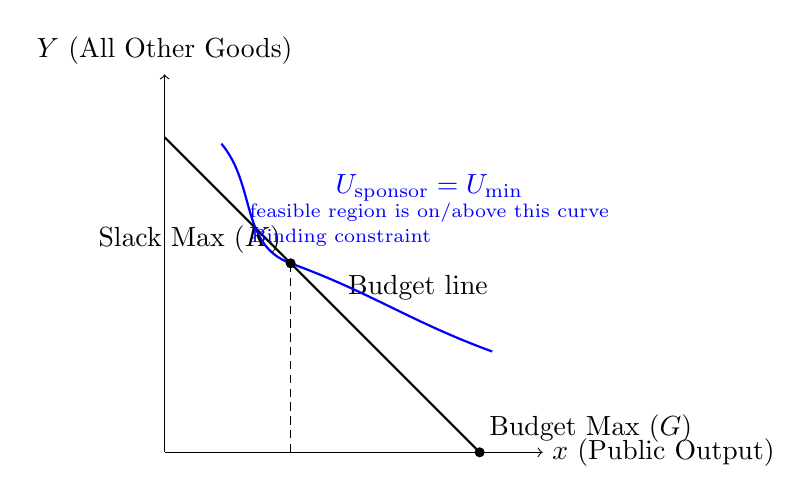
\begin{tikzpicture}[scale=0.8]


\draw[->] (0,0) -- (6,0) node[right] {$x$ (Public Output)};
\draw[->] (0,0) -- (0,6) node[above] {$Y$ (All Other Goods)};


\draw[thick] (0,5) -- (5,0) node[pos=0.55, above right] {Budget line};

\draw[blue, thick]
(0.9,4.9) to[out=-50,in=160] (2,3) to[out=-20,in=160] (5.2,1.6);

\node[blue] at (4.2,4.2) {$U_{\text{sponsor}} = U_{\min}$};
\node[blue] at (4.2,3.8) {\scriptsize feasible region is on/above this curve};

\filldraw (5,0) circle (2pt) node[above right] {Budget Max ($G$)};
\filldraw (2,3) circle (2pt) node[above left] {Slack Max ($K$)};

\node[blue] at (2.8,3.4) {\scriptsize Binding constraint};

\draw[densely dashed] (2,0) -- (2,3);

\end{tikzpicture}

\begin{itemize}
\item \textbf{Budget Max ($G$):} Max output, zero slack.
\item \textbf{Slack Max ($K$):} Lower output, max slack subject to $U_{\text{sponsor}} \ge U_{\min}$ (binding at $K$).
\end{itemize}


\begin{itemize}
\item \textbf{X-axis:} Public output ($Q$).
\item \textbf{Y-axis:} All other goods (resources kept by the sponsor / taxpayers, i.e. money \emph{not} absorbed by the bureau).
\end{itemize}

\textbf{What the diagram is doing}
\begin{itemize}
\item The sponsor values $Q$ but also values keeping resources for other priorities (or lower taxes), so the sponsor’s preferences can be drawn as indifference curves over $(Q,\text{other goods})$.
\item The sponsor requires a minimum acceptable outcome, shown by a reservation indifference curve $U_{\min}$.
\end{itemize}

\framebreak

\textbf{The constraint on the bureau}
\begin{itemize}
\item If the bureau delivers a bundle \emph{below} $U_{\min}$, the sponsor is worse off than its minimum acceptable level and intervenes (cuts budget, restructures, replaces management).
\item So the bureau must choose a point \emph{on or above} $U_{\min}$ to remain in place.
\end{itemize}

\textbf{Where slack enters}
\begin{itemize}
\item For any given output level $Q$, there is a \emph{minimum cost} of producing it.
\item If the bureau receives a budget larger than this minimum cost, the difference is \textbf{slack}:
\[
S \;=\; B \;-\; C_{\min}(Q)
\]
\item A slack-maximiser keeps the sponsor just satisfied (at $U_{\min}$) while choosing production and spending so that slack is as large as possible.
\end{itemize}
The Diagnostic Test: Lump-Sum Grants\\

\textbf{Scenario:} The Central Government gives the Bureau a \$10m "No strings attached" grant.

\textbf{How does the equilibrium shift?}
\begin{itemize}
\item This shifts the Budget Line outward (Parallel shift).
\end{itemize}
\end{frame}

\begin{frame}{Lump-Sum Grant Test}


\begin{center}
\includegraphics[width=0.9\linewidth]{figm.JPG}
\end{center}
\end{frame}


\begin{frame}{Response 1: The Budget Maximizer}
\textbf{Niskanen's Prediction:}
\begin{itemize}
\item The grant reduces the effective "price" of output to the sponsor.
\item The Bureau pushes output until the new budget is exhausted.
\item \textbf{Result:} Massive expansion of Output ($> \$10m$ if elastic).
\end{itemize}
\end{frame}

\begin{frame}{Response 2: The Slack Maximizer}
\textbf{Wyckoff's Prediction:}
\begin{itemize}
\item The Bureau treats the grant as pure income.
\item It keeps output constant (at $K$).
\item It absorbs the entire \$10m as \textbf{Slack} (Perks/Waste).
\item \textbf{Result:} No change in Output. Total Cost rises by exactly \$10m.
\end{itemize}
\end{frame}

\begin{frame}{Evidence: The Flypaper Effect}
\textbf{The Puzzle:} How do local governments spend lump-sum grants?
\vspace{0.3cm}

\begin{columns}[t]
\column{0.48\textwidth}
\textbf{1. Standard Economic Theory:}
\begin{itemize}
\item Money is fungible.
\item A \$10m grant is just extra income for the community.
\item \emph{Prediction:} Local taxes should fall (passing money to citizens).
\end{itemize}

\column{0.48\textwidth}
\textbf{2. Empirical Reality:}
\begin{itemize}
\item \textbf{"Money sticks where it hits."}
\item Spending increases by \$10m; taxes rarely fall.
\item The money stays in the public sector.
\end{itemize}
\end{columns}

\vspace{0.5cm}
\alert{Verdict:} Wyckoff argues this supports the \textbf{Slack Maximizer} model: the bureau absorbs the grant as perks/costs rather than expanding service.
\end{frame}


\begin{frame}{Money Sticks Where It Hits}

\begin{center}
\includegraphics[width=0.9\linewidth]{fign.JPG}
\end{center}
\end{frame}


\section{V. Critique 3: The Bureau-Shaper (Dunleavy)}

\begin{frame}{Dunleavy's Sociological Critique (1985)}
\textbf{Is the Bureau a Monolith?}
\begin{itemize}
\item Niskanen assumes the whole bureau wants the same thing.
\item Dunleavy argues there is a \textbf{Collective Action Problem}. Large organisations have internal politics.
\end{itemize}

\textbf{Divergent Interests:}
\begin{itemize}
\item \textbf{Rank-and-File:} Benefit from budget growth (Job security, promotion).
\item \textbf{Elites (Top Officials):} Do not benefit. Managing a larger bureau means more headaches, more scrutiny, less time for policy.
\end{itemize}
\end{frame}

\begin{frame}{What do Top Bureaucrats Want?}
\textbf{The Elites maximize:}
\begin{itemize}
\item \textbf{Interesting Work:} Policy formulation, strategy.
\item \textbf{Proximity to Power:} Access to Ministers/Politicians.
\item \textbf{Status:} Being part of the "core executive."
\item \textbf{Comfort:} Avoiding industrial relations (strikes) and routine management.
\item Their preferences point toward shaping the organisation, not expanding it.
\end{itemize}
\end{frame}

\begin{frame}{Hierarchical Interests Diverge}

\begin{center}
\includegraphics[width=0.9\linewidth]{figo.JPG}
\end{center} 

\end{frame}

\begin{frame}{The “Hiving Off” Strategy}
\begin{center}
\includegraphics[width=0.9\linewidth]{figp.JPG}
\end{center} 
\end{frame}

\begin{frame}{The Bureau-Shaping Strategy}
\textbf{The Goal:}
Not to maximize the budget, but to \textbf{reshape} the bureau.

\textbf{Strategy: "Hiving Off"}
\begin{itemize}
\item Top bureaucrats actively try to \textbf{shed} routine, risky, or boring functions (e.g., garbage collection, IT services).
\item They push these tasks to:
\begin{itemize}
\item Private contractors (Privatization).
\item Separate agencies (Agencification).
\item Local government.
\end{itemize}
\end{itemize}
\end{frame}




\begin{frame}{Agency Types Matter}
Niskanen's model only fits \textbf{one} type. Dunleavy identifies five:
\begin{enumerate}
\item \textbf{Delivery Agency:} Delivers services (e.g., NHS). Budget Max applies here.
\item \textbf{Regulatory Agency:} Regulates be haviour. Small budget, high power.
\item \textbf{Transfer Agency:} Moves money (e.g., Social Security). No benefit to staff from larger payouts.
\item \textbf{Contract Agency:} Manages tenders.
\item \textbf{Control Agency:} Supervises others (e.g., Treasury). Elites love this.
\end{enumerate}

Dunleavy says: different agency types imply different incentives. The budget-maximisation logic fits best for delivery agencies. But for regulators, control agencies, and transfer agencies, budget size is a poor proxy for what staff want.

\end{frame}

\begin{frame}{Five Agency Types}

\begin{center}
\includegraphics[width=0.9\linewidth]{figq.JPG}
\end{center} 

\end{frame}



\begin{frame}{Prediction: The Regulatory State}
\textbf{Niskanen predicted:} Massive growth of centralized line bureaucracy.
\textbf{Reality:} The rise of the "Hollow State" or "Regulatory State."

\begin{itemize}
\item Central departments stay small and elite (Treasury, Cabinet Office).
\item Service delivery is fragmented/contracted out.
\item This explains the "New Public Management" (NPM) revolution of the 1980s/90s.

\end{itemize}
\end{frame}

\begin{frame}{Discussion Question}
\begin{center}
\large
\textcolor{myOrange}{\textbf{Irish Context:}}
\end{center}

\textbf{Question:} Can you identify examples of "hiving off" or "agencification" in Ireland?

\begin{itemize}
\item Think about services that used to be provided directly by government departments but are now:
\begin{itemize}
\item Contracted to private firms
\item Delivered through semi-state bodies
\item Delegated to local authorities
\end{itemize}
\item Does this fit Dunleavy's bureau-shaping model?
\end{itemize}
\end{frame}

\section{VI. Evidence and The Leviathan}

\begin{frame}{Leviathan (Brennan \& Buchanan)}
\textbf{The Darkest View:}
\begin{itemize}
\item Government is a Revenue-Maximizer (Leviathan).
\item Electoral constraints are weak (Rational Ignorance $\rightarrow$ Voters don’t monitor closely).
\end{itemize}

\textbf{The Constraint: The Constitution}
\begin{itemize}
\item \textbf{Fiscal Federalism:} Competition between regions limits tax rates ("Vote with your feet").
\item \textbf{Tax Base Rules:} Earmarked taxes make costs visible.
\end{itemize}
\end{frame}

\begin{frame}{Empirical Evidence: Public vs. Private (Mueller)}
\textbf{Comparing Costs (Table 16.1):}
\begin{itemize}
\item \textbf{Airlines:} Private 12-100\% more efficient (Davies 1971).
\item \textbf{Refuse Collection:} Public 40-60\% more expensive (Savas 1977).
\item \textbf{Water Utilities:} Public costs 20\% higher (Crain \& Zardkoohi 1978).
\end{itemize}

\alert{Consensus:} Public production is generally less efficient.
\end{frame}

\begin{frame}{Why? Ownership or Competition?}
\textbf{Necessary Distinction:}
\begin{itemize}
\item Is inefficiency due to \textbf{Public Ownership}?
\item Or due to \textbf{Monopoly Status}?
\end{itemize}

\textbf{Nuance:}
\begin{itemize}
\item Private monopolies behave badly too.
\item Public firms in \textbf{competitive} markets (e.g., Renault, Statoil) often behave efficiently.
\item \alert{Competition is the discipline, not just ownership}.
\end{itemize}
\end{frame}

\begin{frame}{Conclusion: The Synthesis}
\textbf{Three Models, Three Insights:}
\begin{enumerate}
\item \textbf{Niskanen:} Incentives lead to \textbf{Oversupply} ($Q > Q^*$).
\item \textbf{Wyckoff/Slack:} Incentives lead to \textbf{Inefficiency} (High Costs).
\item \textbf{Dunleavy:} Incentives lead to \textbf{Complex Structures} (Hiving off).
\end{enumerate}

\textbf{Final Thought:}
\textit{"If you want efficiency, you must design institutions that align the Agent's incentives with the Principal's goals."}
\end{frame}


\section{VII. Modern Applications and Contemporary Context}

\begin{frame}{Digital Government and Information Technology}
\textbf{How has technology changed bureaucratic be haviour?}


\textbf{Reducing Information Asymmetry:}
\begin{itemize}
\item \textbf{Open data portals:} Performance dashboards, spending transparency
\item \textbf{E-government platforms:} Gov.uk, e-Estonia (digital-first delivery)
\item \textbf{Real-time monitoring:} GPS tracking, automated reporting
\end{itemize}


\textbf{New Forms of Bureaucratic Power:}
\begin{itemize}
\item Control over algorithms and data systems
\item Technical expertise becomes more valuable
\item "Digital hiving off" (cloud services, platform dependencies)
\end{itemize}


\alert{Question:} Does technology strengthen or weaken the principal's control?
\end{frame}

\begin{frame}{Be havioural Public Administration}
\textbf{The "Nudge Unit" Revolution (2010s–present)}


\textbf{Example: UK Behavioural Insights Team}
\begin{itemize}
\item Small, elite unit (bureau-shaping model)
\item Low budget, high policy impact
\item Uses be havioural science to improve outcomes without regulation
\end{itemize}


\textbf{Examples of Nudges:}
\begin{itemize}
\item Changing organ donation to opt-out (doubled registration rates)
\item Text message reminders for court appearances, tax payments
\item Simplifying government forms (reduced processing costs)
\end{itemize}


\alert{Implication:} Not all bureaucratic expansion involves budget maximization - some agencies maximize intellectual influence instead.
\end{frame}

\begin{frame}{COVID-19 and Temporary Agencies}
\textbf{Case Study: Emergency Response Bureaucracies}


\textbf{Characteristics:}
\begin{itemize}
\item \textbf{Mission-focused:} Clear objective (pandemic response), not budget maximization
\item \textbf{Temporary:} Built-in sunset clauses (NPHET in Ireland dissolved 2022)
\item \textbf{Cross-departmental:} Broke traditional bureau boundaries
\item \textbf{High urgency:} Reduced information asymmetry (daily reporting, public scrutiny)
\end{itemize}


\textbf{Puzzle for Public Choice Theory:}
\begin{itemize}
\item Why did agencies voluntarily dissolve after pandemic?
\item Suggests organizational mission can override self-interest
\item Or: elites avoided becoming "routine delivery agencies"
\end{itemize}
\end{frame}

\begin{frame}{International Variation in Bureaucratic Performance}

\centering
\textbf{Not all bureaucracies behave the same way}
\vspace{0.3cm}

\begin{columns}[t]
\column{0.48\textwidth}
\begin{exampleblock}{High-Performing Models}
\footnotesize
\begin{itemize}
\item \textbf{Singapore:} High salaries, strict meritocracy
\item \textbf{Nordic Countries:} High trust \& transparency
\item \textbf{Botswana:} Strong institutions
\end{itemize}
\end{exampleblock}

\column{0.48\textwidth}
\begin{block}{Common Features}
\footnotesize
\begin{itemize}
\item Meritocratic recruitment
\item Performance measurement
\item High social status
\item Political stability
\end{itemize}
\end{block}

\end{columns}

\vspace{0.4cm}

\begin{alertblock}{Key Question}
Why do Public Choice pathologies appear stronger in some countries than others?
\end{alertblock}

\end{frame}

\begin{frame}[allowframebreaks]{Limitations of Public Choice Models}
\textbf{Important Caveats:}


\textbf{1. The Self-Interest Assumption}
\begin{itemize}
\item \textbf{Public Service Motivation (PSM):} Many bureaucrats are genuinely motivated by mission, service, civic duty
\item Selection effects: Public sector attracts different personality types than private sector
\end{itemize}


\textbf{2. The Role of Professionalism}
\begin{itemize}
\item Professional norms and ethics constrain opportunism (doctors, teachers, judges)
\item Organizational culture matters (esprit de corps)
\end{itemize}

\framebreak

\textbf{3. Mixed Empirical Evidence}
\begin{itemize}
\item Some public agencies perform exceptionally well (NASA, CDC pre-COVID)
\item Models don't explain cross-country variation
\item Crowding-out effects: Monetary incentives can backfire when intrinsic motivation is high
\end{itemize}


\textbf{4. Oversimplification}
\begin{itemize}
\item Real bureaucrats face multiple principals (legislature, courts, media, interest groups)
\item Career concerns and reputation matter (repeated game dynamics)
\item Not all agencies are monopolies (police forces, universities compete)
\end{itemize}

\framebreak

\textbf{5. Normative Concerns}
\begin{itemize}
\item Market-mimicking reforms can undermine public values (equity, due process)
\item "What gets measured gets managed" - but not everything important is measurable
\item Gaming of performance metrics (teaching to the test, cream-skimming)
\end{itemize}


\alert{Bottom Line:} Public Choice provides valuable insights but should not be the only lens. Institutional context, culture, and professionalism are also important.
\end{frame}

\begin{frame}{Institutional Design: Policy Prescriptions}
\textbf{If bureaucratic incentives are the problem, what's the solution?}


\textbf{Supply-Side Reforms:}
\begin{itemize}
\item \textbf{Performance contracts:} Tie funding to measurable outcomes (New Zealand model)
\item \textbf{Sunset clauses:} Programs automatically expire unless renewed (Texas, Colorado)
\item \textbf{Cost-benefit analysis mandates:} OMB Circular A-4 (US), Green Book (UK)
\item \textbf{Independent audit institutions:} Comptroller \& Auditor General (Ireland), NAO (UK)
\end{itemize}


\textbf{Demand-Side Reforms:}
\begin{itemize}
\item \textbf{Competitive tendering:} Force agencies to bid against private firms
\item \textbf{School choice / vouchers:} Give "customers" exit options
\item \textbf{Fiscal federalism:} Interjurisdictional competition ("voting with feet")
\end{itemize}
\end{frame}

\begin{frame}{Institutional Design (continued)}
\textbf{Transparency Reforms:}
\begin{itemize}
\item \textbf{Freedom of Information Acts:} Reduce information asymmetry (Ireland 2014, UK 2000)
\item \textbf{Open data portals:} Publish spending, performance metrics (data.gov.ie)
\item \textbf{Citizen charters:} Explicit service standards with complaint mechanisms
\end{itemize}


\textbf{Governance Reforms:}
\begin{itemize}
\item \textbf{Arm's length agencies:} Separate policy (political) from delivery (technical)
\item \textbf{Independent regulators:} Insulate technical decisions from politics (Central Bank)
\item \textbf{Third-party monitoring:} Watchdog NGOs, investigative journalism
\end{itemize}


\alert{Trade-offs:} Each reform has costs (compliance burden, gaming, loss of flexibility). No perfect solution exists.
\end{frame}

\begin{frame}{A Matrix: Ownership vs. Competition}
\begin{center}
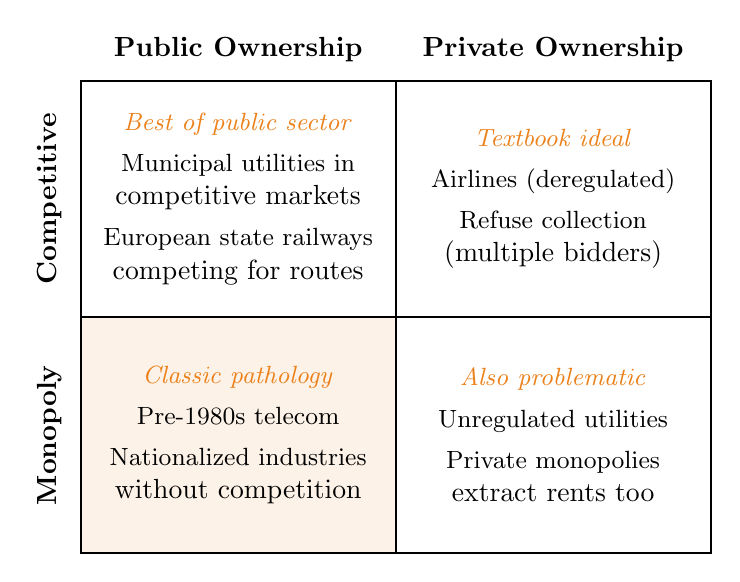
\begin{tikzpicture}[scale=1.0]
\fill[myOrange, opacity=0.10] (0,0) rectangle (4,3);


\draw[thick] (0,0) rectangle (8,6); 
\draw[thick] (4,0) -- (4,6);
\draw[thick] (0,3) -- (8,3);


\node at (2,6.4) {\textbf{Public Ownership}};
\node at (6,6.4) {\textbf{Private Ownership}};


\node[rotate=90] at (-0.4,4.5) {\textbf{Competitive}};
\node[rotate=90] at (-0.4,1.5) {\textbf{Monopoly}};

\node[align=center] at (2,4.5) {\small \textcolor{myOrange}{\textit{Best of public sector}}\\[0.1cm]
\small Municipal utilities in\\competitive markets\\[0.1cm]
\small European state railways\\competing for routes};


\node[align=center] at (6,4.5) {\small \textcolor{myOrange}{\textit{Textbook ideal}}\\[0.1cm]
\small Airlines (deregulated)\\[0.1cm]
\small Refuse collection\\(multiple bidders)};

\node[align=center] at (2,1.5) {\small \textcolor{myOrange}{\textit{Classic pathology}}\\[0.1cm]
\small Pre-1980s telecom\\[0.1cm]
\small Nationalized industries\\without competition};


\node[align=center] at (6,1.5) {\small \textcolor{myOrange}{\textit{Also problematic}}\\[0.1cm]
\small Unregulated utilities\\[0.1cm]
\small Private monopolies\\extract rents too};
\end{tikzpicture}
\end{center}
\alert{Key Insight:} Competition disciplines be haviour more than ownership structure.
\end{frame}




\begin{frame}{Final Synthesis: Where Do We Stand?}
\begin{center}
\begin{tikzpicture}[scale=0.7]

\coordinate (A) at (0,0);
\coordinate (B) at (8,0);
\coordinate (C) at (4,6);


\draw[thick] (A) -- (B) -- (C) -- cycle;


\node[below] at (A) {\textbf{Niskanen (1971)}};
\node[below] at (B) {\textbf{Wyckoff (1990)}};
\node[above] at (C) {\textbf{Dunleavy (1985)}};


\node[align=center, anchor=north] at ($(A)+(0,-0.45)$) {\small Budget Max\\\small \textcolor{myOrange}{\textbf{Allocative Inefficiency}}\\\scriptsize (Doing too much)};
\node[align=center, anchor=north] at ($(B)+(0,-0.45)$) {\small Slack Max\\\small \textcolor{myOrange}{\textbf{Technical Inefficiency}}\\\scriptsize (Doing it expensively)};
\node[align=center, anchor=south] at ($(C)+(0,0.45)$) {\small Bureau-Shaping\\\small \textbf{Structural Change}\\\scriptsize (Hiving Off)};


\node[align=center, fill=white, inner sep=3pt] (reality) at (4,2.5)
{\textbf{Reality:}\\All three operate\\in different contexts};


\draw[->, thick, myOrange] ($(A)+(1,0.6)$) -- (reality);
\draw[->, thick, myOrange] ($(B)+(-1,0.6)$) -- (reality);
\draw[->, thick, myOrange] ($(C)+(0,-1.2)$) -- (reality);
\end{tikzpicture}
\end{center}
\end{frame}



\begin{frame}{Takeaways for Institutional Design}
\begin{enumerate}
\item \textbf{Information asymmetry is the core friction.} Reducing it through transparency, competition, and monitoring is essential.


\item \textbf{Incentives matter, but so does context.} The same reform works differently across agency types, countries, and cultures.


\item \textbf{No single model explains everything.} Budget maximization, slack, bureau-shaping, and public service motivation all coexist.


\item \textbf{Competition is the key discipline.} Ownership matters less than whether agencies face competitive pressure.


\item \textbf{Design institutions, don't rely on virtue.} As Madison wrote: "If men were angels, no government would be necessary." The same applies to bureaucrats.
\end{enumerate}
\end{frame}

\begin{frame}{Final Thought}
\begin{center}
\Large 
"If you put the federal government in charge of the Sahara Desert, \\
in 5 years there'd be a shortage of sand."


\normalsize
- Milton Friedman
\end{center}


\begin{center}
\normalsize
\textbf{But the Public Choice insight is subtler:}\\[0.3cm]
Bureaucrats are not bad people, they just respond rationally to the incentives they face.\\[0.3cm]
\alert{Design better institutions, get better outcomes.}
\end{center}
\end{frame}


\begin{frame}{Summary: The Three Models of Bureaucracy}
\centering
\renewcommand{\arraystretch}{1.5}
\resizebox{\textwidth}{!}{%
\begin{tabular}{l | l | l | l}
\toprule
\textbf{Model} & \textbf{Bureaucrat Wants...} & \textbf{Mechanism} & \textbf{The Problem} \\
\midrule
\textbf{Niskanen} & \textbf{Max Budget} & All-or-Nothing Offer & \textbf{Allocative Inefficiency} \\
(1971) & (Power, Prestige) & (Take it or leave it) & (Too much output) \\
\hline
\textbf{Wyckoff} & \textbf{Max Slack} & Asymmetric Info & \textbf{Technical Inefficiency} \\
(1990) & (Perks, Easy Life) & (Hiding true costs) & (Costs are too high) \\
\hline
\textbf{Dunleavy} & \textbf{Bureau Shaping} & Hiving Off & \textbf{Structural Complexity} \\
(1985) & (Intellectual Interest) & (Delegating boring work) & (Fragmented state) \\
\bottomrule
\end{tabular}
}
\vspace{0.5cm}

\small
\emph{\textbf{Rule of Thumb:} Big Agencies = Niskanen; Wasteful Agencies = Wyckoff; Elite Agencies = Dunleavy.}
\end{frame}

\section{VIII. The Irish Context: Bureaucracy in Practice}

\begin{frame}{Irish Bureaucracy: A Brief Overview}
\textbf{The Irish Civil Service:}

\begin{itemize}
\item \textbf{Size:} Approximately 40,000 civil servants (2024)
\item \textbf{Structure:} 17 government departments
\item \textbf{Tradition:} Strong Weberian foundation (merit-based, professional)
\item \textbf{Reform waves:} Strategic Management Initiative (1990s), Public Service Reform Plan (2011), Civil Service Renewal Plan (2014-2020)
\end{itemize}


\alert{Question:} Which of our three models best explains Irish bureaucracy?
\end{frame}

\begin{frame}{Irish Health Service Executive (HSE): A Case Study}
\textbf{The HSE as a bureaucratic puzzle:}

\begin{itemize}
\item Created 2005 (consolidating 11 health boards)
\item Budget: €24.5 billion (2024) - largest single agency
\item Staff: ~130,000 employees
\end{itemize}


\textbf{Measurement problems:}
\begin{itemize}
\item Observable inputs: staffing levels, beds, procedures
\item Hard-to-measure outputs: population health, patient satisfaction, equity
\item Frequent cost overruns and waiting list controversies
\end{itemize}


\alert{Does this fit Niskanen's budget maximization or Wyckoff's slack model?}
\end{frame}

\begin{frame}{Bureau-Shaping in Ireland: Evidence of Hiving Off}
\textbf{Dunleavy's prediction: Elite bureaucrats "hive off" routine functions}


\textbf{Irish examples:}
\begin{itemize}
\item \textbf{Semi-state bodies:} ESB, Bord Gáis, Irish Water (2014)
\item \textbf{Independent agencies:} Revenue Commissioners, National Transport Authority
\item \textbf{Agencification:} Creation of HIQA (2007), FSPO (2018)
\item \textbf{Privatization:} Eircom (1999), Aer Lingus (partial, 2006)
\item \textbf{PPPs:} M50 toll roads, schools, courthouses
\end{itemize}


\alert{Pattern:} Core departments stay small and strategic; delivery fragmented outward.
\end{frame}

\begin{frame}{Irish Fiscal Institutions: Constraining the Bureaucracy}
\textbf{Post-crisis reforms created new accountability mechanisms:}

\begin{itemize}
\item \textbf{Irish Fiscal Advisory Council (IFAC, 2012):} Independent fiscal watchdog
\item \textbf{Parliamentary Budget Office (2017):} Technical support for Oireachtas
\item \textbf{Rainy Day Fund (2019):} Limits discretionary spending growth
\item \textbf{Performance Budgeting Initiative:} Links outputs to expenditure
\item \textbf{Freedom of Information Acts (1997, 2014):} Transparency requirements
\end{itemize}


\alert{These institutions address the principal-agent problem by reducing information asymmetry.}
\end{frame}

\begin{frame}{Irish Regulatory Agencies: Small Budgets, High Power}
\textbf{Dunleavy's "regulatory agency" type dominates in Ireland:}

\begin{columns}
\column{0.5\textwidth}
\textbf{Examples:}
\begin{itemize}
\item Commission for Regulation of Utilities (CRU)
\item Central Bank of Ireland
\item Competition and Consumer Protection Commission
\item Environmental Protection Agency
\end{itemize}

\column{0.5\textwidth}
\textbf{Characteristics:}
\begin{itemize}
\item Small staff
\item Low budgets
\item High technical expertise
\item Significant regulatory power
\item Elite bureaucrats prefer these roles
\end{itemize}
\end{columns}


\footnotesize
\alert{These agencies fit the bureau-shaping model better than budget maximization.}
\end{frame}

\begin{frame}{The Children's Hospital Saga: Multiple Pathologies}
\textbf{National Children's Hospital (NCH) cost escalation:}
\begin{itemize}
\item \textbf{Original estimate (2014):} €650 million
\item \textbf{Current projection (2024):} €2.2+ billion
\end{itemize}

\vspace{0.3cm}

\begin{block}{The Diagnostic: Which Model Fits?}
\small
\begin{itemize}
\item \textbf{Niskanen (Oversupply):} Is the hospital simply too large/fancy?
\item \textbf{Wyckoff (Slack):} Are we paying too much for inputs (concrete/consultants)?
\item \textbf{Key Concept: The Soft Budget Constraint}
\begin{itemize}
\item The project is "Too Big to Fail."
\item The Agency knows the Govt \emph{must} bail them out.
\item \emph{Result:} No incentive to control costs once construction starts.
\end{itemize}
\end{itemize}
\end{block}

\centering
\alert{Likely a combination of Slack + Soft Budget Constraints.}
\end{frame}


\begin{frame}{Irish Public vs Private Efficiency: Limited Evidence}
\textbf{Comparative data is scarce, but suggestive:}

\begin{itemize}
\item \textbf{Refuse collection:} Mixed public-private provision across local authorities
\item \textbf{Public transport:} Dublin Bus (public) vs private operators
\item \textbf{Healthcare:} Public hospitals vs private/voluntary sector
\end{itemize}


\textbf{A testable student research question:}
\begin{itemize}
\item Compare unit costs of waste collection across Irish local authorities
\item Control for: population density, service quality, geography
\item Test: Does ownership (public/private/contracted) or competition (number of bidders) matter more?
\end{itemize}


\footnotesize
\textit{Data available from: CSO, EPA, local authority annual reports}
\end{frame}

\begin{frame}{Student Research Opportunity: Irish Bureaucratic Growth}
\textbf{Mini-project idea:}

\begin{enumerate}
\item Collect data on:
\begin{itemize}
\item Department employment (2000-2024)
\item Semi-state body creation dates
\item Independent agency establishment
\end{itemize}

\item Test Dunleavy's prediction:
\begin{itemize}
\item Are core departments shrinking or staying stable?
\item Is total public employment growing through agencies/semi-states?
\end{itemize}

\item Compare pre/post financial crisis (2008):
\begin{itemize}
\item Did austerity reverse bureau-shaping?
\item Or accelerate it (more contracting out)?
\end{itemize}
\end{enumerate}


\footnotesize
\textit{Sources: CSO, Department of Public Expenditure \& Reform, Comptroller \& Auditor General reports}
\end{frame}

\begin{frame}{Irish Takeaways}
\textbf{Ireland illustrates the modern bureaucratic landscape:}

\begin{enumerate}
\item \textbf{Budget cycles are limited:} Strong Weberian tradition + post-crisis institutions constrain Niskanen-type be haviour

\item \textbf{Bureau-shaping is evident:} Proliferation of agencies, semi-states, PPPs fits Dunleavy model

\item \textbf{Slack exists but is contested:} Public scrutiny (media, Oireachtas, C\&AG) limits extreme waste

\item \textbf{Information asymmetry persists:} Major projects (NCH, MetroLink) still suffer cost overruns due to measurement/monitoring problems

\item \textbf{Institutions matter:} IFAC, PBO, FOI Acts improve accountability but can't eliminate principal-agent friction
\end{enumerate}
\end{frame}

\section*{Further Reading}

\begin{frame}{Foundational Public Choice Theory of Bureaucracy}
\footnotesize
\begin{enumerate}
\item Niskanen, W. (1971). \emph{Bureaucracy and Representative Government}. Aldine-Atherton.
\item Tullock, G. (1965). \emph{The Politics of Bureaucracy}. Public Affairs Press.
\item Downs, A. (1967). \emph{Inside Bureaucracy}. Little, Brown.
\item Mises, L. von (1944). \emph{Bureaucracy}. Yale University Press.
\item Weber, M. (1922/1978). \emph{Economy and Society}. University of California Press.
\end{enumerate}
\end{frame}

\begin{frame}{Extensions and Critiques of the Niskanen Model}
\footnotesize
\begin{enumerate}
\item Dunleavy, P. (1991). \emph{Democracy, Bureaucracy and Public Choice}. Harvester Wheatsheaf.
\item Wyckoff, P. (1990). "The Simple Analytics of Slack-Maximizing Bureaucracy." \emph{Public Choice}, 67, 35–47.
\item Migué, J.-L., \& Bélanger, G. (1974). "Toward a General Theory of Managerial Discretion." \emph{Public Choice}, 17, 27–43.
\item Miller, G., \& Moe, T. (1983). "Bureaucrats, Legislators, and the Size of Government." \emph{American Political Science Review}, 77(2), 297–322.
\item Breton, A., \& Wintrobe, R. (1982). \emph{The Logic of Bureaucratic Conduct}. Cambridge University Press.
\end{enumerate}
\end{frame}

\begin{frame}{Empirical Studies of Bureaucratic Be haviour}
\footnotesize
\begin{enumerate}
\item Blais, A., \& Dion, S. (1991). \emph{The Budget-Maximizing Bureaucrat}. University of Pittsburgh Press.
\item Mueller, D. (2003). \emph{Public Choice III}, Chapter 16. Cambridge University Press.
\item Rourke, F. (1984). \emph{Bureaucracy, Politics, and Public Policy} (3rd ed.). Little, Brown.
\item Wilson, J.Q. (1989). \emph{Bureaucracy: What Government Agencies Do and Why They Do It}. Basic Books.
\item Hood, C., \& Dixon, R. (2015). \emph{A Government That Worked Better and Cost Less?} Oxford University Press.
\end{enumerate}
\end{frame}

\begin{frame}{Principal-Agent Theory and Information Asymmetry}
\footnotesize
\begin{enumerate}
\item Bendor, J., Taylor, S., \& Van Gaalen, R. (1985). "Bureaucratic Expertise versus Legislative Authority." \emph{American Political Science Review}, 79(4), 1041–1060.
\item McCubbins, M., Noll, R., \& Weingast, B. (1987). "Administrative Procedures as Instruments of Political Control." \emph{Journal of Law, Economics, \& Organization}, 3(2), 243–277.
\item Holmstrom, B., \& Milgrom, P. (1991). "Multitask Principal-Agent Analyses." \emph{Journal of Law, Economics, \& Organization, 7, 24–52}.
\item Epstein, D., \& O'Halloran, S. (1999). \emph{Delegating Powers}. Cambridge University Press.
\item Huber, J., \& Shipan, C. (2002). \emph{Deliberate Discretion?} Cambridge University Press.
\item Gailmard, S., \& Patty, J. (2012). \emph{Learning While Governing}. University of Chicago Press.
\end{enumerate}
\end{frame}

\begin{frame}{Public vs Private Provision: Evidence}
\footnotesize
\begin{enumerate}
\item Savas, E.S. (1977). "Policy Analysis for Local Government: Public vs. Private Refuse Collection." \emph{Policy Analysis}, 3(1), 49–74.
\item Boardman, A., \& Vining, A. (1989). "Ownership and Performance in Competitive Environments." \emph{Journal of Law and Economics}, 32(1), 1–33.
\item Megginson, W., \& Netter, J. (2001). "From State to Market: A Survey of Empirical Studies on Privatization." \emph{Journal of Economic Literature}, 39(2), 321–389.
\item Pollitt, C., \& Bouckaert, G. (2011). \emph{Public Management Reform: A Comparative Analysis} (3rd ed.). Oxford University Press.
\item Hart, O., Shleifer, A., \& Vishny, R. (1997). "The Proper Scope of Government." \emph{Quarterly Journal of Economics}, 112(4), 1127–1161.
\end{enumerate}
\end{frame}

\begin{frame}{New Public Management and Reform}
\footnotesize
\begin{enumerate}
\item Osborne, D., \& Gaebler, T. (1992). \emph{Reinventing Government}. Addison-Wesley.
\item Hood, C. (1991). "A Public Management for All Seasons?" \emph{Public Administration}, 69(1), 3–19.
\item Kettl, D. (2000). \emph{The Global Public Management Revolution}. Brookings Institution.
\item Behn, R. (2001). \emph{Rethinking Democratic Accountability}. Brookings Institution.
\item Christensen, T., \& Lægreid, P. (2011). \emph{The Ashgate Research Companion to New Public Management}. Ashgate.
\end{enumerate}
\end{frame}

\begin{frame}{Bureaucracy and Development}
\footnotesize
\begin{enumerate}
\item Evans, P., \& Rauch, J. (1999). "Bureaucracy and Growth." \emph{American Sociological Review}, 64(5), 748–765.
\item Fukuyama, F. (2013). "What Is Governance?" \emph{Governance}, 26(3), 347–368.
\item Rauch, J., \& Evans, P. (2000). "Bureaucratic Structure and Bureaucratic Performance in Less Developed Countries." \emph{Journal of Public Economics}, 75(1), 49–71.
\item Grindle, M. (2012). \emph{Jobs for the Boys: Patronage and the State in Comparative Perspective}. Harvard University Press.
\item Acemoglu, D., et al. (2021). "(Successful) Democracies Breed Their Own Support." \emph{NBER Working Paper} 29514.
\end{enumerate}
\end{frame}

\begin{frame}{Public Service Motivation and Be havioural Approaches}
\footnotesize
\begin{enumerate}
\item Perry, J., \& Wise, L. (1990). "The Motivational Bases of Public Service." \emph{Public Administration Review}, 50(3), 367–373.
\item Dilulio, J. (1994). "Principled Agents: The Cultural Bases of Be haviour in a Federal Government Bureaucracy." \emph{Journal of Public Administration Research and Theory}, 4(3), 277–318.
\item Besley, T., \& Ghatak, M. (2005). "Competition and Incentives with Motivated Agents." \emph{American Economic Review}, 95(3), 616–636.
\item Prendergast, C. (2007). "The Motivation and Bias of Bureaucrats." \emph{American Economic Review}, 97(1), 180–196.
\item Ashraf, N., \& Bandiera, O. (2018). "Social Incentives in Organizations." \emph{Annual Review of Economics}, 10, 439–463.
\item Hines, J. R., \& Thaler, R. H. (1995). “Anomalies: The Flypaper Effect.” \emph{Journal of Economic Perspectives, 9(4), 217–226}.
\end{enumerate}
\end{frame}

\begin{frame}{Bureaucracy and Regulation}
\footnotesize
\begin{enumerate}
\item Stigler, G. (1971). "The Theory of Economic Regulation." \emph{Bell Journal of Economics}, 2(1), 3–21.
\item Peltzman, S. (1976). "Toward a More General Theory of Regulation." \emph{Journal of Law and Economics}, 19(2), 211–240.
\item Laffont, J.-J., \& Tirole, J. (1991). "The Politics of Government Decision-Making." \emph{Quarterly Journal of Economics}, 106(4), 1089–1127.
\item Carpenter, D. (2001). \emph{The Forging of Bureaucratic Autonomy}. Princeton University Press.
\item Dal Bó, E. (2006). "Regulatory Capture: A Review." \emph{Oxford Review of Economic Policy}, 22(2), 203–225.
\end{enumerate}
\end{frame}

\begin{frame}{Fiscal Institutions and Accountability}
\footnotesize
\begin{enumerate}
\item Von Hagen, J., \& Harden, I. (1995). "Budget Processes and Commitment to Fiscal Discipline." \emph{European Economic Review}, 39(3-4), 771–779.
\item Alesina, A., \& Perotti, R. (1996). "Fiscal Discipline and the Budget Process." \emph{American Economic Review}, 86(2), 401–407.
\item Debrun, X., et al. (2013). "The Functions and Impact of Fiscal Councils." \emph{IMF Policy Paper}.
\item Kopits, G. (2011). "Independent Fiscal Institutions: Developing Good Practices." \emph{OECD Journal on Budgeting}, 11(3), 1–18.
\item Beetsma, R., \& Debrun, X. (2016). "Fiscal Councils: Rationale and Effectiveness." \emph{IMF Working Paper} 16/86.
\end{enumerate}
\end{frame}

\begin{frame}{Irish Context: Specific Studies}
\footnotesize
\begin{enumerate}
\item MacCarthaigh, M. (2017). \emph{Public Sector Reform in Ireland}. Palgrave Macmillan.
\item Hardiman, N., \& MacCarthaigh, M. (2011). "Organizing for Economic Development." In \emph{The Oxford Handbook of Irish Politics}, Oxford University Press.
\item Roche, W., et al. (2016). \emph{Public Service Pay and Pensions in Ireland}. Institute of Public Administration.
\item MacCarthaigh, M., \& Roness, P. (2012). "Analyzing Longitudinal Continuity and Change in Public-Sector Organizations." \emph{International Review of Administrative Sciences}, 78(3), 449–469.
\item Comptroller and Auditor General. Annual Reports (various years). Available at: \href{https://www.audit.gov.ie}{www.audit.gov.ie}
\item Irish Fiscal Advisory Council. \emph{Fiscal Assessment Reports} (2012-present). Available at: \href{https://www.fiscalcouncil.ie}{www.fiscalcouncil.ie}
\end{enumerate}
\end{frame}

\begin{frame}{Contemporary Issues and Digital Government}
\footnotesize
\begin{enumerate}
\item Margetts, H., \& Dunleavy, P. (2013). "The Second Wave of Digital-Era Governance." \emph{Philosophical Transactions of the Royal Society A}, 371.
\item Mergel, I., Edelmann, N., \& Haug, N. (2019). "Defining Digital Transformation." \emph{Government Information Quarterly}, 36(4), 101385.
\item Janssen, M., \& van der Voort, H. (2020). "Agile and Adaptive Governance in Crisis Response." \emph{Government Information Quarterly}, 37(3), 101479.
\item Bannister, F., \& Connolly, R. (2014). "ICT, Public Values and Transformative Government." \emph{Government Information Quarterly}, 31(1), 119–128.
\item OECD (2023). \emph{OECD Framework and Good Practice Principles for People-Centred Justice}. OECD Publishing.
\end{enumerate}
\end{frame}


\section*{Cultural Resources}

\begin{frame}{Films \& Documentaries}
\textbf{Bureaucracy, Power, and Institutions:}
\begin{itemize}
\item \textbf{Yes Minister / Yes Prime Minister} (TV series, 1980-88) – Classic satire on bureau-shaping and bureaucratic power
\item \textbf{The Thick of It} (TV series, 2005-12) – Modern political satire showing principal-agent conflicts
\item \textbf{12 Angry Men} (1957) – Group decision-making and institutional processes
\item \textbf{Erin Brockovich} (2000) – Regulatory capture and bureaucratic failure
\item \textbf{Inside Job} (2010) – Regulatory agencies and the financial crisis
\item \textbf{The Post} (2017) – Whistleblowing and bureaucratic accountability
\end{itemize}
\end{frame}

\begin{frame}{TV Series: Politics and Administration}
\textbf{How bureaucracies actually work:}
\begin{itemize}
\item \textbf{The Wire} (Season 3-4) – Baltimore city bureaucracy, measurement problems
\item \textbf{Borgen} – Civil service vs political leadership in Denmark
\item \textbf{The West Wing} – White House bureaucracy and policy implementation
\item \textbf{Parks and Recreation} – Local government and public service motivation
\item \textbf{Utopia} (Australian) – Infrastructure agencies and cost overruns
\item \textbf{The Office} (UK/US) – Organizational slack and workplace incentives
\end{itemize}
\end{frame}

\begin{frame}{Books for General Audience}
\begin{itemize}
\item \textbf{James C. Scott} – \emph{Seeing Like a State} (1998)
\begin{itemize}
\item How bureaucracies simplify and sometimes fail
\end{itemize}
\item \textbf{Michael Lewis} – \emph{The Fifth Risk} (2018)
\begin{itemize}
\item What government agencies actually do
\end{itemize}
\item \textbf{Jennifer Pahlka} – \emph{Recoding America} (2023)
\begin{itemize}
\item Digital transformation in government
\end{itemize}
\item \textbf{David Graeber} – \emph{The Utopia of Rules} (2015)
\begin{itemize}
\item Bureaucracy and modern life
\end{itemize}
\item \textbf{Francis Fukuyama} – \emph{Political Order and Political Decay} (2014)
\begin{itemize}
\item State capacity and bureaucratic quality
\end{itemize}
\end{itemize}
\end{frame}

\begin{frame}{Irish Context: Books and Reports}
\textbf{Understanding Irish public administration:}
\begin{itemize}
\item \textbf{Muiris MacCarthaigh} – \emph{Public Sector Reform in Ireland} (2017)
\item \textbf{Tom Garvin} – \emph{Preventing the Future} (2004)
\begin{itemize}
\item How Irish bureaucracy shaped development
\end{itemize}
\item \textbf{Comptroller \& Auditor General Reports}
\begin{itemize}
\item Real examples of bureaucratic performance (www.audit.gov.ie)
\end{itemize}
\item \textbf{IFAC Fiscal Assessment Reports}
\begin{itemize}
\item Fiscal institutions in action (www.fiscalcouncil.ie)
\end{itemize}
\end{itemize}
\end{frame}

\begin{frame}[allowframebreaks]{Podcasts \& Media}
\textbf{Public Administration and Policy:}
\begin{itemize}
\item \textbf{EconTalk} – Episodes on bureaucracy, regulation, public choice
\item \textbf{Planet Money} – Government programs and incentives
\item \textbf{Freakonomics Radio} – Be havioural economics in government
\item \textbf{99\% Invisible} – Design and infrastructure (bureaucracy in action)
\item \textbf{Working} (Slate) – How government workers actually work
\end{itemize}

\framebreak
\textbf{Irish Policy and Politics:}
\begin{itemize}
\item \textbf{Inside Politics} (RTÉ) – Irish political economy
\item \textbf{The Business} (RTÉ) – Public sector and regulation
\item \textbf{Oireachtas TV/Radio} – Committee hearings (bureaucratic accountability in real time)
\end{itemize}

\framebreak
\textbf{Data and Transparency:}
\begin{itemize}
\item \textbf{Our World in Data} – Cross-country government effectiveness
\item \textbf{The Economist – Democracy Index}
\item \textbf{Transparency International} – Corruption perceptions
\item \textbf{World Bank – Worldwide Governance Indicators}
\end{itemize}
\end{frame}

\begin{frame}{Case Studies: Real Bureaucratic Puzzles}
\textbf{Use these to test the models:}

\begin{enumerate}
\item \textbf{NASA:} High-performing agency despite government ownership
\begin{itemize}
\item What institutional features explain this?
\end{itemize}

\item \textbf{UK's National Health Service:} Persistent efficiency debates
\begin{itemize}
\item Budget max, slack, or measurement problems?
\end{itemize}

\item \textbf{Singapore Civil Service:} High pay, high performance
\begin{itemize}
\item How do incentives differ from typical bureaucracies?
\end{itemize}

\item \textbf{Irish Water controversy (2014-2017):}
\begin{itemize}
\item Bureau-shaping gone wrong? Political backlash to agencification?
\end{itemize}
\end{enumerate}
\end{frame}

\section*{Appendices}

\begin{frame}{Appendix A: Deriving the Budget Maximizer (1/3)}
\textbf{The Bureaucrat's Optimization Problem}

The Bureau wants to maximize its total budget $B(Q)$, subject to the constraint that the budget must cover total costs $C(Q)$.

\[
\max_{Q} B(Q) \quad \text{subject to} \quad B(Q) \ge C(Q)
\]

\vspace{0.5cm}

\textbf{Step 1: The Lagrangian Function}
We set up the Lagrangian ($\mathcal{L}$) with a multiplier $\lambda$ (representing the "shadow price" or tightness of the constraint):

\[
\mathcal{L} = B(Q) + \lambda [ B(Q) - C(Q) ]
\]

\end{frame}


\begin{frame}{Appendix A: Deriving the Budget Maximizer (2/3)}
\textbf{Step 2: First-Order Condition (F.O.C.)}
To find the maximum, we take the partial derivative with respect to Output ($Q$) and set it to zero:

\[
\frac{\partial \mathcal{L}}{\partial Q} = B'(Q) + \lambda [ B'(Q) - C'(Q) ] = 0
\]

\vspace{0.3cm}

\textbf{Step 3: Rearranging terms}
We group the marginal benefit terms $B'(Q)$:

\[
(1 + \lambda) B'(Q) - \lambda C'(Q) = 0
\]

Moving the cost term to the right-hand side gives us the equilibrium condition:

\[
\alert{(1 + \lambda) B'(Q) = \lambda C'(Q)}
\]

\end{frame}


\begin{frame}{Appendix A: Economic Interpretation (3/3)}
\textbf{Step 4: Interpreting the Multiplier ($\lambda$)}
Solving for Marginal Benefit:
\[
B'(Q) = \frac{\lambda}{1 + \lambda} C'(Q)
\]

\begin{itemize}
\item Since the Bureau spends its entire budget, the constraint is \textbf{binding}, so $\lambda > 0$.
\item This implies that the fraction $\frac{\lambda}{1+\lambda} < 1$.
\end{itemize}

\vspace{0.3cm}

\textbf{Conclusion: Allocative Inefficiency}
\[
\implies B'(Q) < C'(Q)
\]

At the bureau's equilibrium, the \textbf{Marginal Benefit} of the last unit produced is \textbf{less} than its \textbf{Marginal Cost}. The bureau has expanded output into the region of negative net value (waste).
\end{frame}

\begin{frame}{Appendix B: Elasticity and Budget Revenue (1/2)}
\textbf{Deriving the Revenue Change Condition}

If the Bureau sets a price $P$ for its services, the total budget is:
\[
B(P) = P \cdot Q(P)
\]

\textbf{Step 1: Differentiate with respect to Price ($P$)}
Using the Product Rule ($uv' + vu'$):
\[
\frac{dB}{dP} = 1 \cdot Q(P) + P \cdot \frac{dQ}{dP}
\]

\textbf{Step 2: Factor out Quantity ($Q$)}
To find elasticity, we factor out $Q$ from the right-hand side:
\[
\frac{dB}{dP} = Q \left[ 1 + \frac{P}{Q} \frac{dQ}{dP} \right]
\]

\end{frame}


\begin{frame}{Appendix B: Elasticity and Budget Revenue (2/2)}
\textbf{Step 3: Substitute Price Elasticity of Demand ($\eta$)}
Recall the standard definition of elasticity (absolute value):
\[
\eta = \left| \frac{\%\Delta Q}{\%\Delta P} \right| = - \frac{dQ}{dP} \cdot \frac{P}{Q}
\]
Rearranging terms implies that $\frac{P}{Q} \frac{dQ}{dP} = -\eta$.

\vspace{0.3cm}

\textbf{Step 4: The Final Condition}
Substitute $-\eta$ back into the budget equation:
\[
\alert{\frac{dB}{dP} = Q [ 1 - \eta ]}
\]

\textbf{Conclusion:}
\begin{itemize}
\item \textbf{Elastic ($\eta > 1$):} The term $[1-\eta]$ is negative. $\frac{dB}{dP} < 0$ (Budget shrinks).
\item \textbf{Inelastic ($\eta < 1$):} The term $[1-\eta]$ is positive. $\frac{dB}{dP} > 0$ (Budget grows).
\end{itemize}
\end{frame}

\end{document}